

%\url{https://github.com/cedrict/fieldstone/tree/master/python_codes/fieldstone_56}

Saltwater intrusion in coastal aquifers is a world wide observable phenomena. The mixing of salt and fresh water reduces groundwater quality. It potentially threatens the usability as drinking water. Extensive pumping causing a decrease of groundwater levels amplifies this effect. 


Gravity drives salty sea water land inward due to its higher density if an aquifer's water table is lower than sea level.
An interface develops between salt and fresh water, which is stable due to the density difference. Along the interface slight mixing occurs due to diffusion.
As for most processes in nature, coupled partial differential equations describe the movement of the interface between salt and fresh water. 

The target of this exercise is to model a simplified form of the process. Basic assumption hereby are: (i) groundwater flow is mostly horizontal (called {\sl Depuit assumption}); 
(ii) the salt and fresh water interface is sharp, meaning we neglect mixing due to dispersion and diffusion. 


We investigate a portion of an aquifer of length $L$ and depth $H$. Within the aquifer, an interface separates salt water and fresh water as illustrated here under:

\begin{center}
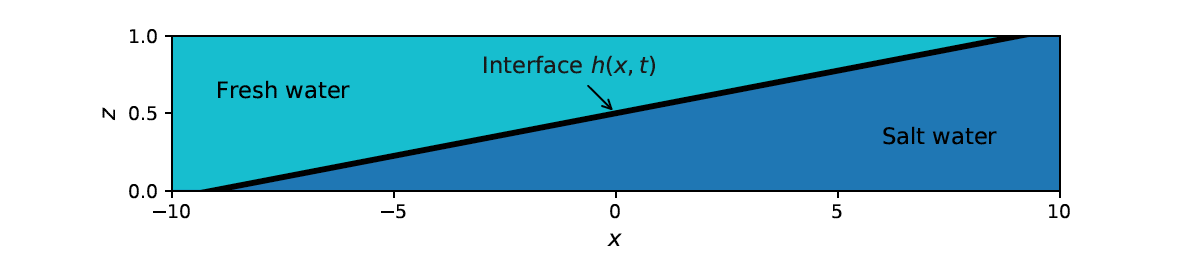
\includegraphics[width=13cm]{python_codes/fieldstone_56/images/setup}
\end{center}

The interface~$h(x,t)$ is a function of the horizontal location~$x$ and time~$t$. 
For simplicity, we assume an aquifer thickness of $H=1$. Thus, the values for the position of the interface as a function in the $z$ direction range between zero and one: $h(x,t) \in [0,1]$.

The differential equation describing the movement of the interface $h(x,t)$ is given by 

\begin{equation} \label{eq:01}
	\frac{\partial h(x,t)}{\partial t} = \Gamma \frac{\partial}{\partial x} \left( \frac{ h(1-h)\partial h / \partial x}{1+(\partial h/\partial x)^2} \right)
\end{equation}

The constant $\Gamma=\frac{\kappa }{ \mu g (\rho_{ \rm salt}-\rho_{\rm fresh})}$ summarizes the physical properties: of the aquifer (permeability $\kappa$), of the fluids (viscosity $\mu$, density of salt water~$\rho_{\rm salt}$ and density of fresh water~$\rho_{\rm fresh}$) and the gravity constant $g$.

The differential equation has the character of a non-linear diffusion equation with a non-constant diffusion coefficient $D(h)$:

\begin{equation} \label{eq:02}
	\frac{\partial h}{\partial t} = \Gamma \frac{\partial}{\partial x} \left( D(h)  \frac{ \partial h}{\partial x} \right)
	\quad \quad D(h(x,t)) = \frac{ h(1-h)}{1+(\partial h/\partial x)^2}
\end{equation}

According to the value range of $h \in [0,1]$, $D$ has the property of $D(0)=D(1)=0$ (this differential equation is therefore called {\sl degenerate}). \index{stones}{Degenerate Diffusion Equation}

Despite the complexity of the initial differential equation, an analytical solution can be postulated in the form of:
\begin{equation}  \label{eq:04}
	h(x,t) = a(t)\cdot x + 0.5
\end{equation}

The interface $h$ is a linear function in $x$ with a time-dependent slope~$a(t)$. It rotates with time around the fix point~$(0;0.5)$. 
The slope~$a(t)$ can be determined by the ordinary differential equation (REF??):
\begin{equation}  \label{eq:05}
\frac{ da(t) }{dt} = - \frac{2a^3}{1+a^2}
\end{equation}

The value range of $a$ is limited to $0<a(t)<1$ corresponding to a maximal slope angle of $45^\circ$. The differential equation in $a(t)$ has an implicit solution:
\begin{equation} \label{eq:05b}
t = \frac 1 2 \ln \left( \frac{a(0)}{a(t)} \right) + \frac 1 4 \left( \frac{1}{a(t)^2} - \frac{1}{a(0)^2} \right)
\end{equation}

We aim to implement a numerical solution of the differential equation 1 which allows us to calculate the location of the interface $h(x,t)$ at specified locations $x$ and times $t$.

{\Huge To Do} in 2D only



